\documentclass[12pt]{article}
\usepackage[utf8]{inputenc}
\usepackage{amsmath}
\usepackage{graphicx}
\usepackage{multicol}
\usepackage{fancyhdr}

\usepackage[
    left=2.5cm,
    right=2.5cm,
    top=4cm,
    bottom=4cm
]{geometry}
\setlength{\parindent}{0em}

\setlength{\headheight}{15.0pt}
\pagestyle{fancy}
\lhead{18.06 Lectures 6-10}
\chead{Alisa Ono}
\rhead{January 2018}

\begin{document}

\section{Column Space and Nullspace (L6)}

\subsection{Column Space}

Given a $4\times3$ matrix $A$ whose columns are in $R^4$ space:

\[
A=
\left(
    \begin{matrix}
        1 & 1 & 2\\ 
        2 & 1 & 3\\
        3 & 1 & 4\\
        4 & 1 & 5\\
    \end{matrix}
\right)
\]

Column space $C(A)$ is the linear combination of $A$'s columns, which forms a subspace of $R^4$.

\[
C(A)=
c_1
\left(
    \begin{matrix}
        1\\ 
        2\\
        3\\
        4\\
    \end{matrix}
\right)
+ c_2
\left(
    \begin{matrix}
        1\\ 
        1\\
        1\\
        1\\
    \end{matrix}
\right)
+ c_3
\left(
    \begin{matrix}
        2\\ 
        3\\
        4\\
        5\\
    \end{matrix}
\right)
\]

\textbf{Does $Ax=b$ have a solution for every $b$?}

\[
Ax=
\left(
    \begin{matrix}
        1 & 1 & 2\\ 
        2 & 1 & 3\\
        3 & 1 & 4\\
        4 & 1 & 5\\
    \end{matrix}
\right)
\left(
    \begin{matrix}
        x_1\\ 
        x_2\\
        x_3\\
    \end{matrix}
\right)
=
\left(
    \begin{matrix}
        b_1\\ 
        b_2\\
        b_3\\
        b_4\\
    \end{matrix}
\right)
=b
\]

No, because there are 4 equations and 3 unknowns.

$\>$

\textbf{Which $b$ allows the system to be solved?}

\[
\text{e.g.}
\quad
b=
\left(
    \begin{matrix}
        0\\ 
        0\\
        0\\
        0\\
    \end{matrix}
\right)
\Rightarrow
x=
\left(
    \begin{matrix}
        0\\ 
        0\\
        0\\
    \end{matrix}
\right)
\quad
b=
\left(
    \begin{matrix}
        1\\ 
        2\\
        3\\
        4\\
    \end{matrix}
\right)
\Rightarrow
x=
\left(
    \begin{matrix}
        1\\ 
        0\\
        0\\
    \end{matrix}
\right)
\]

$Ax=b$ is solvable if $b$ is the linear combination of $A$'s columns i.e. $C(A)$

\subsection{Null Space}
\[
Ax=
\left(
    \begin{matrix}
        1 & 1 & 2\\ 
        2 & 1 & 3\\
        3 & 1 & 4\\
        4 & 1 & 5\\
    \end{matrix}
\right)
\left(
    \begin{matrix}
        x_1\\ 
        x_2\\
        x_3\\
    \end{matrix}
\right)
=
\left(
    \begin{matrix}
        0\\ 
        0\\
        0\\
        0\\
    \end{matrix}
\right)
\]

Null space $N(A)$ is all the solutions $x$ to $Ax=0$, which forms a subspace of $R^3$.

\begin{multicols}{2}
{\[
x=c
\left(
    \begin{matrix}
        1\\ 
        1\\
        -1\\
    \end{matrix}
\right)
\]}

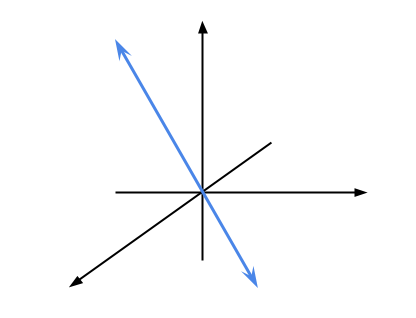
\includegraphics[width=\linewidth]{6-1}
\end{multicols}

If $Av=0$ and $Aw=0$, then $A(c_1v+c_2w)=c_1Av+c_2Aw=0$, therefore \textbf{solutions to $Ax=0$ always give a subspace.}

\newpage

\section{$Ax = 0$, Special Solutions, Reduced Row Form (L7)}

\subsection{Example: Solving $Ax=0$}

Given a matrix $A$ for 3 equations and 4 unknowns:

\[
A=
\left(
    \begin{matrix}
        1 & 2 & 2 & 2\\ 
        2 & 4 & 6 & 8\\
        3 & 6 & 8 & 10\\
    \end{matrix}
\right)
\]

Third row of $A$ is dependent on the first and second i.e. $r_3 = r_1 + r_2$. Second column of $A$ is dependent on the first i.e. $c_2 = 2c_1$.

$\>$

Run eliminations to derive $U$ in an echelon (staircase) form:

\[
\left(
    \begin{matrix}
        \boxed{1} & 2 & 2 & 2\\ 
        2 & 4 & 6 & 8\\
        3 & 6 & 8 & 10\\
    \end{matrix}
\right)
\Rightarrow
\left(
    \begin{matrix}
        \boxed{1} & 2 & 2 & 2\\ 
        2-2*1 & 4-2*2 & 6-2*2 & 8-2*2\\
        3-3*1 & 6-3*2 & 8-3*2 & 10-3*2\\
    \end{matrix}
\right)
=
\left(
    \begin{matrix}
        \boxed{1} & 2 & 2 & 2\\ 
        0 & 0 & 2 & 4\\
        0 & 0 & 2 & 4\\
    \end{matrix}
\right)
\]

\[
\left(
    \begin{matrix}
        \boxed{1} & 2 & 2 & 2\\ 
        0 & 0 & \boxed{2} & 4\\
        0 & 0 & 2 & 4\\
    \end{matrix}
\right)
\Rightarrow
\left(
    \begin{matrix}
        \boxed{1} & 2 & 2 & 2\\ 
        0 & 0 & \boxed{2} & 4\\
        0-0 & 0-0 & 2-2 & 4-4\\
    \end{matrix}
\right)
=
\left(
    \begin{array}{*{4}{c}}
        \boxed{1} & 2 & 2 & 2\\
        \cline{1-2}
        0 & \multicolumn{1}{c|}{0} & \boxed{2} & 4\\
        \cline{3-4}
        0 & 0 & 0 & 0\\
    \end{array}
\right)
=U
\]

$\>$

\begin{itemize}
    \item Pivot Column: $c_1$ and $c_3$
    \item Pivot Rows: $r_1$ and $r_2$
    \item Free Columns: $c_2$ and $c_4$ $\Rightarrow$ Any values can be assigned to $x_2$ and $x_4$
    \item Rank $r$: Number of pivots = 2 (1 at $U_{11}$ and 2 at $U_{23}$)
    \item Number of free variables: $n-r=4-2=2$ ($x_2$ and $x_4$)
\end{itemize}

Equations we have are:

\[ 
\left \{
  \begin{tabular}{ccccc}
  $x_1$ & $+2x_2$ & $+2x_3$ & $+2x_4$ & $=0$\\
  & & $2x_3$ & $+4x_4$ & $=0$\\
  \end{tabular}
\right
.\]

We can assign specific values to $x_2$ and $x_4$ and solve equations to derive $x_1$ and $x_3$. We'll call these special solutions:

\[ 
\left \{
  \begin{tabular}{cc}
  $x_2$ & $=1$\\
  $x_4$ & $=0$\\
  \end{tabular}
\right
.\Rightarrow
\left \{
  \begin{tabular}{cc}
  $x_1$ & $=-2$\\
  $x_3$ & $=0$\\
  \end{tabular}
\right
.\quad
\left \{
  \begin{tabular}{cc}
  $x_2$ & $=0$\\
  $x_4$ & $=1$\\
  \end{tabular}
\right
.\Rightarrow
\left \{
  \begin{tabular}{cc}
  $x_1$ & $=2$\\
  $x_3$ & $=-2$\\
  \end{tabular}
\right
.\]

Null space (all solutions to $Ax=0$) is the linear combination of the special solutions:

\[
N(A)=c
\left(
    \begin{matrix}
        -2\\
        1\\
        0\\
        0\\
    \end{matrix}
\right)
+d
\left(
    \begin{matrix}
        2\\
        0\\
        -2\\
        1\\
    \end{matrix}
\right)
\]

\subsection{Reduced Row Echelon Form (RREF)}

Matrix is in a RREF when all pivots are 1s and there are all 0s below and above the pivots.

For example, starting with $U$ from the previous section:
\[
U=
\left(
    \begin{matrix}
        \boxed{1} & 2 & 2 & 2\\
        0 & 0 & \boxed{2} & 4\\
        0 & 0 & 0 & 0\\
    \end{matrix}
\right)
\]

\[
\Rightarrow
\left(
    \begin{matrix}
        1-0=1 & 2-0=2 & 2-2=0 & 2-4=-2\\
        0 & 0 & 2 & 4\\
        0 & 0 & 0 & 0\\
    \end{matrix}
\right)
\Rightarrow
\left(
    \begin{matrix}
        1 & 2 & 0 & -2\\
        0/2=0 & 0=0 & 2/2=1 & 4/2=2\\
        0 & 0 & 0 & 0\\
    \end{matrix}
\right)
\]

\[
R=RREF(A)=
\left(
    \begin{matrix}
        \boxed{1} & 2 & 0 & -2\\
        0 & 0 & \boxed{1} & 2\\
        0 & 0 & 0 & 0\\
    \end{matrix}
\right)
\]

Notice how the pivot columns and rows of $R$ forms an identity matrix $I$:

\[
\left(
    \begin{array}{*{4}{c}}
    \cline{1-1}\cline{3-3}
    \multicolumn{1}{|c|}{1} & 2 & \multicolumn{1}{|c|}{0} & -2\\
    \multicolumn{1}{|c|}{0} & 0 & \multicolumn{1}{|c|}{1} & 2\\
    \cline{1-1}\cline{3-3}
    0 & 0 & 0 & 0\\
    \end{array}
\right)
\Rightarrow
    \begin{array}{*{2}{c}}
    \cline{1-2}
    \multicolumn{1}{|c|}{1} & \multicolumn{1}{c|}{0}\\
    \multicolumn{1}{|c|}{0} & \multicolumn{1}{c|}{1}\\
    \cline{1-2}
    \end{array}
=I
\]

Similarly the free columns and rows of $R$ forms a matrix $F$:

\[
\left(
    \begin{array}{*{4}{c}}
    \cline{2-2}\cline{4-4}
    1 & \multicolumn{1}{|c|}{2} & 0 & \multicolumn{1}{|c|}{-2}\\
    0 & \multicolumn{1}{|c|}{0} & 1 & \multicolumn{1}{|c|}{2}\\
    \cline{2-2}\cline{4-4}
    0 & 0 & 0 & 0\\
    \end{array}
\right)
\Rightarrow
    \begin{array}{*{2}{c}}
    \cline{1-2}
    \multicolumn{1}{|c|}{2} & \multicolumn{1}{c|}{-2}\\
    \multicolumn{1}{|c|}{0} & \multicolumn{1}{c|}{2}\\
    \cline{1-2}
    \end{array}
=F
\]

Those matrices $I$ and $F$ form the special solutions from the previous section:

\[
\left(
    \begin{matrix}
        -2\\
        \boxed{1}\\
        0\\
        \boxed{0}\\
    \end{matrix}
\right)
\left(
    \begin{matrix}
        2\\
        \boxed{0}\\
        -2\\
        \boxed{1}\\
    \end{matrix}
\right)
\Rightarrow
    \begin{array}{*{2}{c}}
    \cline{1-2}
    \multicolumn{1}{|c|}{1} & \multicolumn{1}{c|}{0}\\
    \cline{1-2}
    \multicolumn{1}{|c|}{0} & \multicolumn{1}{c|}{1}\\
    \cline{1-2}
    \end{array}
=I
\quad
\left(
    \begin{matrix}
        \boxed{-2}\\
        1\\
        \boxed{0}\\
        0\\
    \end{matrix}
\right)
\left(
    \begin{matrix}
        \boxed{2}\\
        0\\
        \boxed{-2}\\
        1\\
    \end{matrix}
\right)
\Rightarrow
    \begin{array}{*{2}{c}}
    \cline{1-2}
    \multicolumn{1}{|c|}{-2} & \multicolumn{1}{c|}{2}\\
    \cline{1-2}
    \multicolumn{1}{|c|}{0} & \multicolumn{1}{c|}{-2}\\
    \cline{1-2}
    \end{array}
=-F
\]

$\>$

In general, $R$ ($A$ in RREF) can be broken down into $I$, $F$, and zeros. $I$ and $F$ form the null space matrix $N$ i.e. the columns of $I$ and $F$ form special solutions.

\[
Rx=
\left(
    \begin{matrix}
        I & F
    \end{matrix}
\right)
\left(
    \begin{matrix}
        x_{pivot}\\
        x_{free}\\
    \end{matrix}
\right)
=0
\]

\[
x_{pivot} = -Fx_{free}
\Rightarrow
\left \{
  \begin{tabular}{ccc}
  $x_{pivot}$ & $=$ & $-F$\\
  $x_{free}$ & $=$ & $I$\\
  \end{tabular}
\right
.
\]

\[
RN=0
\Rightarrow
N=x=
\left(
    \begin{matrix}
        -F\\
        I\\
    \end{matrix}
\right)
\]

\subsection{Additional Example}

Eliminations from $A$ to $U$:

\[
A=
\left(
    \begin{matrix}
        \boxed{1} & 2 & 3\\
        2 & 4 & 6\\
        2 & 6 & 8\\
        2 & 8 & 10\\
    \end{matrix}
\right)
\Rightarrow
\left(
    \begin{matrix}
        \boxed{1} & 2 & 3\\
        0 & \boxed{0} & 0\\
        0 & 2 & 2\\
        0 & 4 & 4\\
    \end{matrix}
\right)
\Rightarrow
\left(
    \begin{matrix}
        \boxed{1} & 2 & 3\\
        0 & \boxed{2} & 2\\
        0 & 0 & 0\\
        0 & 4 & 4\\
    \end{matrix}
\right)
\Rightarrow
\left(
    \begin{matrix}
        \boxed{1} & 2 & 3\\
        0 & \boxed{2} & 2\\
        0 & 0 & 0\\
        0 & 0 & 0\\
    \end{matrix}
\right)
=U
\]

\begin{itemize}
    \item Pivot columns: $c_1$ and $c_2$ $\Rightarrow$ Rank = 2
    \item Free columns: $c_3$
\end{itemize}

Assign $x_3=1$:

\[
\left \{
  \begin{tabular}{cccc}
  $x_1$ & $+2x_2$ & $+3x_3$ & $=0$\\
  & $2x_2$ & $+2x_3$ & $=0$\\
  \end{tabular}
\right
.\Rightarrow
\left \{
  \begin{tabular}{cc}
  $x_1$ & $=-1$\\
  $x_2$ & $=-1$\\
  \end{tabular}
\right
.\Rightarrow
x=c
\left(
    \begin{matrix}
        -1\\
        -1\\
        1\\
    \end{matrix}
\right)
=N(A)
\]

Eliminations from $U$ to $R$:

\[
U=
\left(
    \begin{matrix}
        \boxed{1} & 2 & 3\\
        0 & \boxed{2} & 2\\
        0 & 0 & 0\\
        0 & 0 & 0\\
    \end{matrix}
\right)
\Rightarrow
\left(
    \begin{matrix}
        \boxed{1} & 0 & 1\\
        0 & \boxed{2} & 2\\
        0 & 0 & 0\\
        0 & 0 & 0\\
    \end{matrix}
\right)
\Rightarrow
\left(
    \begin{matrix}
        \boxed{1} & 0 & 1\\
        0 & \boxed{1} & 1\\
        0 & 0 & 0\\
        0 & 0 & 0\\
    \end{matrix}
\right)
=R
\]

\newpage

\section{Solving $Ax = b$ (L8)}

Is there a solution? Is the solution unique?

\[
\left \{
  \begin{tabular}{ccccc}
  $x_1$ & $+2x_2$ & $+2x_3$ & $+2x_4$ & $=b_1$\\
  $2x_1$ & $+4x_2$ & $+6x_3$ & $+8x_4$ & $=b_2$\\
  $3x_1$ & $+6x_2$ & $+8x_3$ & $+10x_4$ & $=b_3$\\
  \end{tabular}
\right
.\Rightarrow
Ax=
\left(
    \begin{matrix}
        1 & 2 & 2 & 2\\
        2 & 4 & 6 & 8\\
        3 & 6 & 8 & 10\\
    \end{matrix}
\right)
\left(
    \begin{matrix}
        x_1\\
        x_2\\
        x_3\\
        x_4\\
    \end{matrix}
\right)
=
\left(
    \begin{matrix}
        b_1\\
        b_2\\
        b_3\\
    \end{matrix}
\right)
\]

Run eliminations on an augmented matrix 
$\left(
    \begin{array}{c|c}
        A & b
    \end{array}
\right)$
until the left side is in an echelon form:

\[
\left(
    \begin{array}{cccc|c}
        \boxed{1} & 2 & 2 & 2 & b_1\\ 
        2 & 4 & 6 & 8 & b_2\\
        3 & 6 & 8 & 10 & b_3\\
    \end{array}
\right)
\Rightarrow
\left(
    \begin{array}{cccc|c}
        \boxed{1} & 2 & 2 & 2 & b_1\\ 
        0 & 0 & \boxed{2} & 4 & b_2 - 2b_1\\
        0 & 0 & 2 & 4 & b_3 - 3b_1\\
    \end{array}
\right)
\Rightarrow
\left(
    \begin{array}{cccc|c}
        \boxed{1} & 2 & 2 & 2 & b_1\\ 
        0 & 0 & \boxed{2} & 4 & b_2 - 2b_1\\
        0 & 0 & 0 & 0 & b_3 - b_2 - b_1\\
    \end{array}
\right)
\]

The third row shows the equations are solvable if $b_3 - b_2 - b_1 = 0$ e.g.  
$b=
\left(
    \begin{matrix}
        1\\
        5\\
        6\\
    \end{matrix}
\right)
$

\textbf{Solvability}

$\>$

$Ax=b$ is solvable when $b$ is in $C(A)$. If a combination of $A$'s rows give a zero row, some combination of $b$'s entries must also give zero.

\subsection{Complete Solution for $Ax=b$}

Find the particular solution $x_p$ by setting all free variables to 0s and solving $Ax=b$ for pivot variables:

\[
\left \{
  \begin{tabular}{cccccc}
  $x_1$ & $+2x_2$ & $+2x_3$ & $+2x_4$ & $=$ & $b_1$\\
  & & $+2x_3$ & $+4x_4$ & $=$ & $b_2-2b_1$\\
  \end{tabular}
\right
.\quad
b=
\left(
    \begin{matrix}
        1\\
        5\\
        6\\
    \end{matrix}
\right)
\]

\[
\left \{
  \begin{tabular}{c}
  $x_2=0$\\
  $x_4=0$\\
  \end{tabular}
\right
.\Rightarrow
\left \{
  \begin{tabular}{c}
  $x_1=-2$\\
  $x_3=\frac{3}{2}$\\
  \end{tabular}
\right
.\]

\[
x_p=
\left(
    \begin{matrix}
        -2\\
        0\\
        \frac{3}{2}\\
        0\\
    \end{matrix}
\right)
\]

Complete solution for $Ax=b$ is a combination of $x_p$ and the null space $x_n$:

\[
Ax_p=b
\quad
Ax_n=0
\quad
\Rightarrow
\quad
A(x_p+x_n)=b
\]

\[
x_{complete}=
x_p + x_n = 
\left(
    \begin{matrix}
        -2\\
        0\\
        \frac{3}{2}\\
        0\\
    \end{matrix}
\right)
+c_1
\left(
    \begin{matrix}
        -2\\
        1\\
        0\\
        0\\
    \end{matrix}
\right)
+c_2
\left(
    \begin{matrix}
        2\\
        0\\
        -2\\
        1\\
    \end{matrix}
\right)
\]

\subsection{Full Ranks}

$A$ is a $m\times{n}$ matrix with rank $r$ $\Rightarrow$ $r\leq{m},r\leq{n}$

$\>$

\textbf{Full Column Rank:} $r=n<m$

\[
A=
\left(
    \begin{matrix}
        1 & 3\\
        2 & 1\\
        6 & 1\\
        5 & 1\\
    \end{matrix}
\right)
\Rightarrow
R=
\left(
    \begin{matrix}
        1 & 0\\
        0 & 1\\
        0 & 0\\
        0 & 0\\
    \end{matrix}
\right)
\]

\begin{itemize}
    \item Every column is a pivot column. No free columns.
    \item Null space $N(A)$ contains only the zero vector.
    \item $Ax=b$ 0 or 1 solutions, depending on $b$.
    \item If $Ax=b$ has a solution, $x=x_p$ i.e. unique solution.
\end{itemize}

\textbf{Full Row Rank:} $r=m<n$

\[
A=
\left(
    \begin{matrix}
        1 & 2 & 6 & 5\\
        3 & 1 & 1 & 1\\
    \end{matrix}
\right)
\Rightarrow
R=
\left(
    \begin{matrix}
        1 & 0 & - & -\\
        0 & 1 & - & -\\
    \end{matrix}
\right)
\]

\begin{itemize}
    \item $m$ pivot columns, $n-m$ free columns.
    \item $Ax=b$ has $\infty$ solutions for any $b$.
\end{itemize}

\textbf{Square Full Rank:} $r=m=n$

\[
A=
\left(
    \begin{matrix}
        1 & 2\\
        3 & 1\\
    \end{matrix}
\right)
\Rightarrow
R=
\left(
    \begin{matrix}
        1 & 0\\
        0 & 1\\
    \end{matrix}
\right)
\]

\begin{itemize}
    \item $R$ is an identity matrix.
    \item $Ax=b$ has 1 solution for any given $b$.
\end{itemize}

\begin{center}
  \begin{tabular}{|c|c|c|}
    \hline
    $r,m,n$ & Number of Solutions & $R$ \\ \hline
    $r=n=m$ & 1 & 
    $\left(\begin{matrix}
        I\\
    \end{matrix}\right)$ \\ \hline
    $r=n<m$ & 0 or 1 &
    $\left(\begin{matrix}
        I\\
        0\\
    \end{matrix}\right)$ \\ \hline
    $r=m<n$ & $\infty$ &
    $\left(\begin{matrix}
        I & F\\
    \end{matrix}\right)$ \\ \hline
    $r<m,n$ & 0 or $\infty$ &    
    $\left(\begin{matrix}
        I & F\\
        0 & 0\\
    \end{matrix}\right)$ \\ \hline
  \end{tabular}
\end{center}

\newpage

\section{Independence, Basis, Dimension (L9)}

Suppose $m<n$ for a $m\times{n}$ matrix $A$, there are non-zero solutions to $Ax=0$. Why?

\begin{itemize}
    \item More unknowns than equations.
    \item There will be free variables.
\end{itemize}

\subsection{Independence}

Vectors $x_1,x_2,...,x_n$ are \underline{independent} if no combination gives a zero vector except when all coefficients are zeros:

\[
c_1x_1 + c_2x_2 + ... + c_nx_n \neq 0 \quad \text{if $c_i \neq 0$ for some $i$}
\]

\begin{center}
    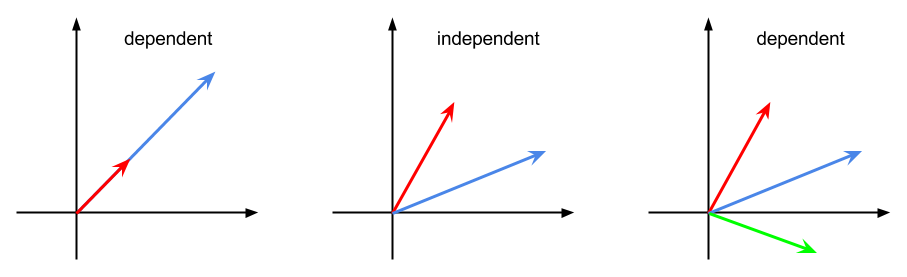
\includegraphics[width=0.8\linewidth]{9-1}
\end{center}

Given $A$'s columns consist of $x_1,x_2,...,x_n$:

\[
A=
\left(
    \begin{matrix}
        x_1 & x_2 & ... & x_n\\
        x_1 & x_2 & ... & x_n\\
    \end{matrix}
\right)
\]

If $x_1,x_2,...,x_n$ are independent:

\[
\left(
    \begin{matrix}
        x_1 & x_2 & ... & x_n\\
        x_1 & x_2 & ... & x_n\\
    \end{matrix}
\right)
\left(
    \begin{matrix}
        c_1\\
        c_2\\
        c_3\\
    \end{matrix}
\right)
=
\left(
    \begin{matrix}
        0\\
        0\\
    \end{matrix}
\right)
\quad \text{only if}
\quad
\left \{
  \begin{tabular}{cc}
  $c_1$ & $=0$\\
  $c_2$ & $=0$\\
  $c_3$ & $=0$
  \end{tabular}
\right.
\]

In other words, they are independent if $N(A)$ contains only the zero vector i.e. $rank(A)<n$ and there are no free variables. They're dependent if $Ac=0$ for some non-zero $c$.

\subsection{Span}

Vectors $x_1,x_2,...,x_n$ \underline{span} a space when the space consists of all combinations of those vectors.

\subsection{Basis}

Vectors $x_1,x_2,...,x_n$ are \underline{basis} for a space when they are independent \textit{and} span the space.

Standard basis for space $R^3$ is:

\[
\left(
    \begin{matrix}
        1\\
        0\\
        0\\
    \end{matrix}
\right)
\quad
\left(
    \begin{matrix}
        0\\
        1\\
        0\\
    \end{matrix}
\right)
\quad
\left(
    \begin{matrix}
        0\\
        0\\
        1\\
    \end{matrix}
\right)
\]

Another example of basis for space $R^3$ is:

\[
\left(
    \begin{matrix}
        1\\
        1\\
        2\\
    \end{matrix}
\right)
\quad
\left(
    \begin{matrix}
        2\\
        2\\
        5\\
    \end{matrix}
\right)
\quad
\left(
    \begin{matrix}
        3\\
        8\\
        1\\
    \end{matrix}
\right)
\]

\begin{itemize}
    \item Basis of $R^n$: $n$ vectors give basis of $R^n$ if $n\times{n}$ matrix with those columns is invertable.
    \item Given a space, every basis for the space has the same number of vectors. This number is the \underline{dimension} of the space.
\end{itemize}

\subsection{Example}

\[
A=
\left(
    \begin{matrix}
        1 & 2 & 3 & 1\\
        1 & 1 & 2 & 1\\
        1 & 2 & 3 & 1\\
    \end{matrix}
\right)
\quad
N(A)=
\left(
    \begin{matrix}
        -1\\
        -1\\
        1\\
        0\\
    \end{matrix}
\right)
\]

Given the space $C(A)$: Column vectors of $A$ span the space.

There are 2 pivot columns because only the first and second columns are independent. Therefore rank of $A$ i.e. dimension of $C(A)$ is 2.

$\>$

One example of basis for $C(A)$:

\[
2
\left(
    \begin{matrix}
        1\\
        1\\
        1\\
    \end{matrix}
\right)
\quad
\left(
    \begin{matrix}
        1\\
        1\\
        1\\
    \end{matrix}
\right)
+2
\left(
    \begin{matrix}
        3\\
        2\\
        3\\
    \end{matrix}
\right)
\quad
\Rightarrow
\quad
\left(
    \begin{matrix}
        2\\
        2\\
        2\\
    \end{matrix}
\right)
\quad
\left(
    \begin{matrix}
        7\\
        5\\
        7\\
    \end{matrix}
\right)
\]

They are independent, both in $C(A)$. We need two vectors since the dimension is 2.

$\>$

Now given the space $N(A)$ instead, the dimension of $N(A)$ i.e. number of free variables is 2. 

One example of basis for $N(A)$:
$\left(
    \begin{matrix}
        -1\\
        -1\\
        1\\
        0\\
    \end{matrix}
\right)
\quad
\left(
    \begin{matrix}
        -1\\
        0\\
        0\\
        1\\
    \end{matrix}
\right)$

\newpage

\section{The Four Fundamental Subspaces (L10)}

Given a $m\times{n}$ matrix $A$:

\begin{itemize}
    \item Column space $C(A)$ in $R^m$
    \item Null space $N(A)$ in $R^n$
    \item Row space = All combinations of $A$'s rows i.e. $A^T$'s columns = $C(A^T)$ in $R^n$
    \item Null space of $A^T$ = $N(A^T)$ in $R^m$
\end{itemize}

\begin{center}
  \begin{tabular}{|c|c|c|c|}
    \hline
    & Space & Basis & Dimension \\ \hline
    $C(A)$ & $R^m$ & pivot columns & $rank(A)=r$ \\ \hline
    $N(A^T)$ & $R^m$ & & $m-r$ \\ \hline
    Row space & $R^n$ & & $r$ \\ \hline 
    $N(A)$ & $R^n$ & special solutions & $n-r$ \\ \hline
  \end{tabular}
\end{center}

\subsection{Row Space Example}

\[
A=
\left(
    \begin{matrix}
        1 & 2 & 3 & 1\\
        1 & 1 & 2 & 1\\
        1 & 2 & 3 & 1\\
    \end{matrix}
\right)
\Rightarrow
\left(
    \begin{matrix}
        1 & 2 & 3 & 1\\
        0 & -1 & -1 & 0\\
        0 & 0 & 0 & 0\\
    \end{matrix}
\right)
\Rightarrow
\left(
    \begin{matrix}
        1 & 2 & 3 & 1\\
        0 & 1 & 1 & 0\\
        0 & 0 & 0 & 0\\
    \end{matrix}
\right)
\Rightarrow
\left(
    \begin{matrix}
        \boxed{1} & 0 & 1 & 1\\
        0 & \boxed{1} & 1 & 0\\
        0 & 0 & 0 & 0\\
    \end{matrix}
\right)
=R
\]

\begin{itemize}
    \item Different column spaces: $C(A) \neq C(R)$
    \item Same row spaces: $R(A) = R(R)$
    \item Basis for row space is the first $r$ rows of $R$
\end{itemize}

\subsection{Null Space of $A^T$}

\[
A^{T}y=0
\quad
\Rightarrow
\quad
y^{T}A^{TT}=y^{T}A=0^T
\]

\[
rref(
\left(
    \begin{array}{c|c}
        A_{m\times{n}} & I_{m\times{m}}
    \end{array}
\right)
)=E
\left(
    \begin{array}{c|c}
        A_{m\times{n}} & I_{m\times{m}}
    \end{array}
\right)
=
\left(
    \begin{array}{c|c}
        R_{m\times{n}} & E_{m\times{m}}
    \end{array}
\right)
\]

\[
\text{e.g.}\quad
EA=
\left(
    \begin{array}{*{3}{c}}
        -1 & 2 & 0\\
        1 & -1 & 0\\
        \cline{1-3}
        \multicolumn{1}{|c}{-1} & 0 & \multicolumn{1}{c|}{1}\\
        \cline{1-3}
    \end{array}
\right)
\left(
    \begin{matrix}
        1 & 2 & 3 & 1\\
        1 & 1 & 2 & 1\\
        1 & 2 & 3 & 1\\
    \end{matrix}
\right)
=
\left(
    \begin{array}{*{4}{c}}
        1 & 0 & 1 & 1\\
        0 & 1 & 1 & 0\\
        \cline{1-4}
        \multicolumn{1}{|c}{0} & 0 & 0 & \multicolumn{1}{c|}{0}\\
        \cline{1-4}
    \end{array}
\right)
=R
\]

Third row of $E$ is the combination of rows that gives zeros i.e. $y^T$

\end{document}
